%%%%%%%%%%%%%%%%%%%%%%%%%%%%%%%%%%%%%%%%%
% Programming/Coding Assignment
% LaTeX Template
%
% This template has been downloaded from:
% http://www.latextemplates.com
%
% Original author:
% Ted Pavlic (http://www.tedpavlic.com)
%
% Note:
% The \lipsum[#] commands throughout this template generate dummy text
% to fill the template out. These commands should all be removed when 
% writing assignment content.
%
% This template uses a Perl script as an example snippet of code, most other
% languages are also usable. Configure them in the "CODE INCLUSION 
% CONFIGURATION" section.
%
%%%%%%%%%%%%%%%%%%%%%%%%%%%%%%%%%%%%%%%%%

%----------------------------------------------------------------------------------------
%	PACKAGES AND OTHER DOCUMENT CONFIGURATIONS
%----------------------------------------------------------------------------------------

\documentclass[a4paper]{article}
\usepackage[utf8]{inputenc}
\usepackage{listingsutf8}
\usepackage[spanish]{babel}




\usepackage{fancyhdr} % Required for custom headers
\usepackage{lastpage} % Required to determine the last page for the footer
\usepackage{extramarks} % Required for headers and footers
\usepackage[usenames,dvipsnames]{color} % Required for custom colors
\usepackage{graphicx} % Required to insert images
\usepackage{listings} % Required for insertion of code
\usepackage{courier} % Required for the courier font
\usepackage{lipsum} % Used for inserting dummy 'Lorem ipsum' text into the template
\usepackage{svg}
\usepackage{attachfile}
\usepackage{currfile}
\usepackage{multicol}
\usepackage{alltt}
\usepackage{framed}
\usepackage{caption}
\usepackage{seqsplit}

\hypersetup{
colorlinks,
citecolor=black,
filecolor=black,
linkcolor=black,
urlcolor=blue
}


% Margins
\topmargin=-0.45in
\evensidemargin=0in
\oddsidemargin=0in
\textwidth=6.5in
\textheight=9.8in
\headsep=0.25in

\linespread{1.1} % Line spacing
\setlength{\parindent}{1.5em}
\setlength{\parskip}{1em}


% Set up the header and footer
\pagestyle{fancy}
%\lhead{\hmwkAuthorName} % Top left header
\lhead{\hmwkClass}
\rhead{\hmwkTitle} % Top right header
\chead{} % Top center head
\lfoot{\lastxmark} % Bottom left footer
\cfoot{} % Bottom center footer
\rfoot{ \thepage\ / \protect\pageref{LastPage}} % Bottom right footer
\renewcommand\headrulewidth{0.4pt} % Size of the header rule
\renewcommand\footrulewidth{0.4pt} % Size of the footer rule



%----------------------------------------------------------------------------------------
%	CODE INCLUSION CONFIGURATION
%----------------------------------------------------------------------------------------
\renewcommand{\ttdefault}{pcr}
\definecolor{MyDarkGreen}{rgb}{0.0,0.4,0.0} % This is the color used for comments
\lstloadlanguages{Perl} % Load Perl syntax for listings, for a list of other languages supported see: ftp://ftp.tex.ac.uk/tex-archive/macros/latex/contrib/listings/listings.pdf
\lstset{
language=sh, % Use Perl in this example
frame=single, % Single frame around code
basicstyle=\small\ttfamily, % Use small true type font
keywordstyle=[1]\small\color{Blue}\bf, % Perl functions bold and blue
keywordstyle=[2]\small\color{Purple}, % Perl function arguments purple
keywordstyle=[3]\small\color{Blue}\underbar, % Custom functions underlined and blue
identifierstyle=, % Nothing special about identifiers                                         
commentstyle=\small\color{MyDarkGreen}, % Comments small dark green courier font
stringstyle=\small\color{Purple}, % Strings are purple
showstringspaces=false, % Don't put marks in string spaces
tabsize=5, % 5 spaces per tab
morecomment=[l][\small\color{Blue}]{...}, % Line continuation (...) like blue comment
numbers=none, % Line numbers on left
firstnumber=1, % Line numbers start with line 1
numberstyle=\tiny\color{Blue}, % Line numbers are blue and small
stepnumber=0 % Line numbers go in steps of 5
}

% Creates a new command to include a perl script, the first parameter is the filename of the script (without .pl), the second parameter is the caption
\newcommand{\perlscript}[2]{
\begin{itemize}
\item[]\lstinputlisting[caption=#2,label=#1]{#1.pl}
\end{itemize}
}

%----------------------------------------------------------------------------------------
%	DOCUMENT STRUCTURE COMMANDS
%	Skip this unless you know what you're doing
%----------------------------------------------------------------------------------------

% Header and footer for when a page split occurs within a problem environment
\newcommand{\enterProblemHeader}[1]{
%\nobreak\extramarks{#1}{#1 continued on next page\ldots}\nobreak
%\nobreak\extramarks{#1 (continued)}{#1 continued on next page\ldots}\nobreak
}

% Header and footer for when a page split occurs between problem environments
\newcommand{\exitProblemHeader}[1]{
%\nobreak\extramarks{#1 (continued)}{#1 continued on next page\ldots}\nobreak
%\nobreak\extramarks{#1}{}\nobreak
}

\setcounter{secnumdepth}{0} % Removes default section numbers
\newcounter{homeworkProblemCounter} % Creates a counter to keep track of the number of problems

\newcommand{\homeworkProblemName}{}
\newenvironment{homeworkProblem}[1][]{ % Makes a new environment called homeworkProblem which takes 1 argument (custom name) but the default is "Problem #"
\stepcounter{homeworkProblemCounter} % Increase counter for number of problems
\renewcommand{\homeworkProblemName}{Ejercicio \arabic{homeworkProblemCounter} #1} % Assign \homeworkProblemName the name of the problem
\section{\homeworkProblemName} % Make a section in the document with the custom problem count
\enterProblemHeader{\homeworkProblemName} % Header and footer within the environment
}{
\exitProblemHeader{\homeworkProblemName} % Header and footer after the environment
%\clearpage
}


\newcommand{\problemAnswer}[1]{ % Defines the problem answer command with the content as the only argument
\noindent\framebox[\columnwidth][c]{\begin{minipage}{0.98\columnwidth}#1\end{minipage}} % Makes the box around the problem answer and puts the content inside
}

\newcommand{\homeworkSectionName}{}
\newenvironment{homeworkSection}[1]{ % New environment for sections within homework problems, takes 1 argument - the name of the section
\renewcommand{\homeworkSectionName}{#1} % Assign \homeworkSectionName to the name of the section from the environment argument
\subsection{\homeworkSectionName} % Make a subsection with the custom name of the subsection
\enterProblemHeader{\homeworkProblemName\ [\homeworkSectionName]} % Header and footer within the environment
}{
\enterProblemHeader{\homeworkProblemName} % Header and footer after the environment
}

%----------------------------------------------------------------------------------------
%	NAME AND CLASS SECTION
%----------------------------------------------------------------------------------------

\newcommand{\hmwkTitle}{Redefine el hmwkTitle} % Assignment title
\newcommand{\hmwkDueDate}{asdfadsf} % Due date
\newcommand{\hmwkClass}{Redefine hmwkClass} % Course/class
\newcommand{\hmwkClassTime}{} % Class/lecture time
\newcommand{\hmwkClassInstructor}{} % Teacher/lecturer
\newcommand{\hmwkAuthorName}{Álvaro González Sotillo} % Your name

%----------------------------------------------------------------------------------------
%	TITLE PAGE
%----------------------------------------------------------------------------------------

\title{
\vspace{2in}
\textmd{\textbf{\hmwkClass:\ \hmwkTitle}}\\
\vspace{0.1in}\large{\textit{\hmwkClassInstructor\ \hmwkClassTime}}
\vspace{3in}
}

\author{\textbf{\hmwkAuthorName}}
\date{} % Insert date here if you want it to appear below your name


%----------------------------------------------------------------------------------------

\usepackage{fancybox}
\newcommand{\codigo}[1]{\texttt{#1}}


% CUADRITO
\newsavebox{\fmboxx}
\newenvironment{cuadrito}[1][14cm]
{\noindent \begin{center} \begin{lrbox}{\fmboxx}\noindent\begin{minipage}{#1}}
{\end{minipage}\end{lrbox}\noindent\shadowbox{\usebox{\fmboxx}} \end{center}}





\newenvironment{entradasalida}[2][14cm]
{
  \newcommand{\elnombredelafiguradeentradasalida}{#2}
  \begin{figure}[h]
    \begin{cuadrito}[#1]
      \begin{scriptsize}
\begin{alltt}
}
{%
\end{alltt}%
      \end{scriptsize}%
    \end{cuadrito}%
    \caption{\elnombredelafiguradeentradasalida}
  \end{figure}
}


\newenvironment{entradasalidacols}[2][14cm]
{
\newcommand{\elnombredelafiguradeentradasalida}{#2}
%\begin{wrapfigure}{}{0.1}
\begin{cuadrito}[#1]
\begin{scriptsize}
\begin{alltt}
}
{
\end{alltt}
\end{scriptsize}
\end{cuadrito}
\captionof{figure}{\elnombredelafiguradeentradasalida}
%\end{wrapfigure}
}


\usepackage{pgffor}
\newcommand{\ficheroautoref}[0]{%
  \foreach \ficherotex in {../../../common/plantilla-ejercicio.tex,../../common/plantilla-ejercicio.tex,../common/plantilla-ejercicio.tex,../apuntes/common/plantilla-ejercicio.tex}{

    \IfFileExists{\ficherotex}%
    {%
      \textattachfile[mimetype=text/plain,%
      description={La plantilla},%
      subject={La plantilla}]%
      {\ficherotex}%
      {}%
      % RECUPERO ESPACIO VERTICAL PERDIDO
      \vspace{-6em}%
    }%
    {}%
  }
  

  \textattachfile[mimetype=text/plain,
  description={El fichero TEX original para crear este documento, no sea que se nos pierda},
  subject={El fichero TEX original para crear este documento, no sea que se nos pierda}]
  {\currfilename}{}

}

\newcommand{\entradausuario}[1]{\textit{\textbf{#1}}}

\newcommand{\enlace}[2]{\textcolor{blue}{{\href{#1}{#2}}}}

\newcommand{\adjuntarfichero}[3]{
\textattachfile[mimetype=text/plain,
color={0 0 0},
description={#3},
subject={#1}]
{#1}
{\textcolor{blue}{\codigo{#2}}}
}

\newcommand{\adjuntardoc}[2]{%
\textattachfile[mimetype=text/plain,%
color={0 0 0},%
description={#1},%
subject={#1}]%
{#1}%
{\textcolor{blue}{#2}}%
}%


\newcommand{\plantilladeclase}[2]{
\adjuntarfichero{#1.java}{#2}{Plantilla para la clase #2}
}

% https://en.wikibooks.org/wiki/LaTeX/Source_Code_Listings#Encoding_issue
\lstset{literate=
  {á}{{\'a}}1 {é}{{\'e}}1 {í}{{\'i}}1 {ó}{{\'o}}1 {ú}{{\'u}}1
  {Á}{{\'A}}1 {É}{{\'E}}1 {Í}{{\'I}}1 {Ó}{{\'O}}1 {Ú}{{\'U}}1
  {à}{{\`a}}1 {è}{{\`e}}1 {ì}{{\`i}}1 {ò}{{\`o}}1 {ù}{{\`u}}1
  {À}{{\`A}}1 {È}{{\'E}}1 {Ì}{{\`I}}1 {Ò}{{\`O}}1 {Ù}{{\`U}}1
  {ä}{{\"a}}1 {ë}{{\"e}}1 {ï}{{\"i}}1 {ö}{{\"o}}1 {ü}{{\"u}}1
  {Ä}{{\"A}}1 {Ë}{{\"E}}1 {Ï}{{\"I}}1 {Ö}{{\"O}}1 {Ü}{{\"U}}1
  {â}{{\^a}}1 {ê}{{\^e}}1 {î}{{\^i}}1 {ô}{{\^o}}1 {û}{{\^u}}1
  {Â}{{\^A}}1 {Ê}{{\^E}}1 {Î}{{\^I}}1 {Ô}{{\^O}}1 {Û}{{\^U}}1
  {œ}{{\oe}}1 {Œ}{{\OE}}1 {æ}{{\ae}}1 {Æ}{{\AE}}1 {ß}{{\ss}}1
  {ű}{{\H{u}}}1 {Ű}{{\H{U}}}1 {ő}{{\H{o}}}1 {Ő}{{\H{O}}}1
  {ç}{{\c c}}1 {Ç}{{\c C}}1 {ø}{{\o}}1 {å}{{\r a}}1 {Å}{{\r A}}1
  {€}{{\euro}}1 {£}{{\pounds}}1 {«}{{\guillemotleft}}1
  {»}{{\guillemotright}}1 {ñ}{{\~n}}1 {Ñ}{{\~N}}1 {¿}{{?`}}1
}

\lstset{
  inputencoding=utf8,
  captionpos=b,
  frame=single,
  basicstyle=\small\ttfamily,
  showstringspaces=false,
  numbers=none,
  numbers=left,
  xleftmargin=2em,
  breaklines=true,
  postbreak=\mbox{\textcolor{red}{$\hookrightarrow$}\space}
}

\renewcommand{\lstlistingname}{Listado}
\captionsetup[lstlisting]{font={footnotesize},labelfont=bf,position=bottom}
\captionsetup[figure]{font={footnotesize},labelfont=bf}
\lstnewenvironment{listadojava}[2]
{
  \lstset{language=Java,caption={#1},label={#2}}
  \noindent\minipage{\linewidth}%
}
{\endminipage}

% LISTADO SHELL
\lstnewenvironment{listadoshell}[2]
{
  \lstset{language=bash,caption={#1},label={#2}}
  \noindent\minipage{\linewidth}%
}
{\endminipage}

% LISTADO TXT
\lstnewenvironment{listadotxt}[2]
{
  \lstset{caption={#1},label={#2}, keywords={}}
  \noindent\minipage{\linewidth}%
}
{\endminipage}

% LISTADO SQL
\lstnewenvironment{listadosql}[2]%
{%
  %(el 1 )caption es #1\\%
  %(el 2) label es #2\\%
  \lstset{language=sql,caption={#1},label={#2}}%
  \noindent\minipage{\linewidth}%
}
{\endminipage}
  






\newcommand{\graficosvg}[3][14cm]{
\begin{figure}[htbp]
\centering
\textattachfile{#2.svg}{
\color{black}
\includesvg[width=#1]{#2}
}
\caption{#3}
\end{figure}
}


\newcommand{\graficosvguml}[3][7cm]{
  \texttt{\graficosvg[#1]{#2}{#3}}
}


\newcommand{\primerapagina}{
\newpage
\ficheroautoref
\tableofcontents
\newpage
}

% CAJAS
\usepackage[skins]{tcolorbox}
\newtcolorbox{Aviso}[1][Aviso]{
  enhanced,
  colback=gray!5!white,
  colframe=gray!75!black,fonttitle=\bfseries,
  colbacktitle=gray!85!black,
  attach boxed title to top left={yshift=-2mm,xshift=2mm},
  title=#1
}


\newcommand{\StudentData}{
  \begin{cuadrito}[1\textwidth]
    \vspace{0.3cm}
    \large{
      \textbf{Apellidos:} \hrulefill \\
      \textbf{Nombre:} \hrulefill \\
      \textbf{Fecha:} \hrulefill \hspace{1cm} \textbf{Grupo:} \hrulefill \\
    }
    %\vspace{0.2cm}
  \end{cuadrito}
}

% TEXTO EN MONOESPACIO PERO QUE SE PARTE EN LINEAS
\usepackage{seqsplit}
\newcommand{\tecnico}[1]{\texttt{\seqsplit{#1}}}

% REEMPLAZAR TEXTO, NO LO USO
\def\replace#1#2#3{%
 \def\tmp##1#2{##1#3\tmp}%
   \tmp#1\stopreplace#2\stopreplace}
\def\stopreplace#1\stopreplace{}

\usepackage{eurosym}


\renewcommand{\hmwkClass}{Planificación y Administración de Redes}
\renewcommand{\hmwkTitle}{Práctica VLAN en Cisco}




\begin{document}

% \maketitle

% ----------------------------------------------------------------------------------------
%	TABLE OF CONTENTS
% ----------------------------------------------------------------------------------------

% \setcounter{tocdepth}{1} % Uncomment this line if you don't want subsections listed in the ToC

\primerapagina

\setlength{\parindent}{0em}
\setlength{\parskip}{1em}


\section{Objetivo de la práctica}
Los objetivos de la práctica son:
\begin{itemize}
\item Comprender los conceptos necesarios para implantar una VLAN
\item Configurar un router con NAT para exponer un servicio
\item Configurar una VPN con SSH
\item Ayudarse de un acceso remoto auxiliar
\end{itemize}


La última versión de esta práctica está disponible en \enlace{https://alvarogonzalezsotillo.github.io/apuntes-clase/planificacion-administracion-redes-asir1/apuntes/8/par-8-vpn-ssh.pdf}{este enlace}.


\section{Diagrama general}

\begin{figure}[h]
  \begin{center}
    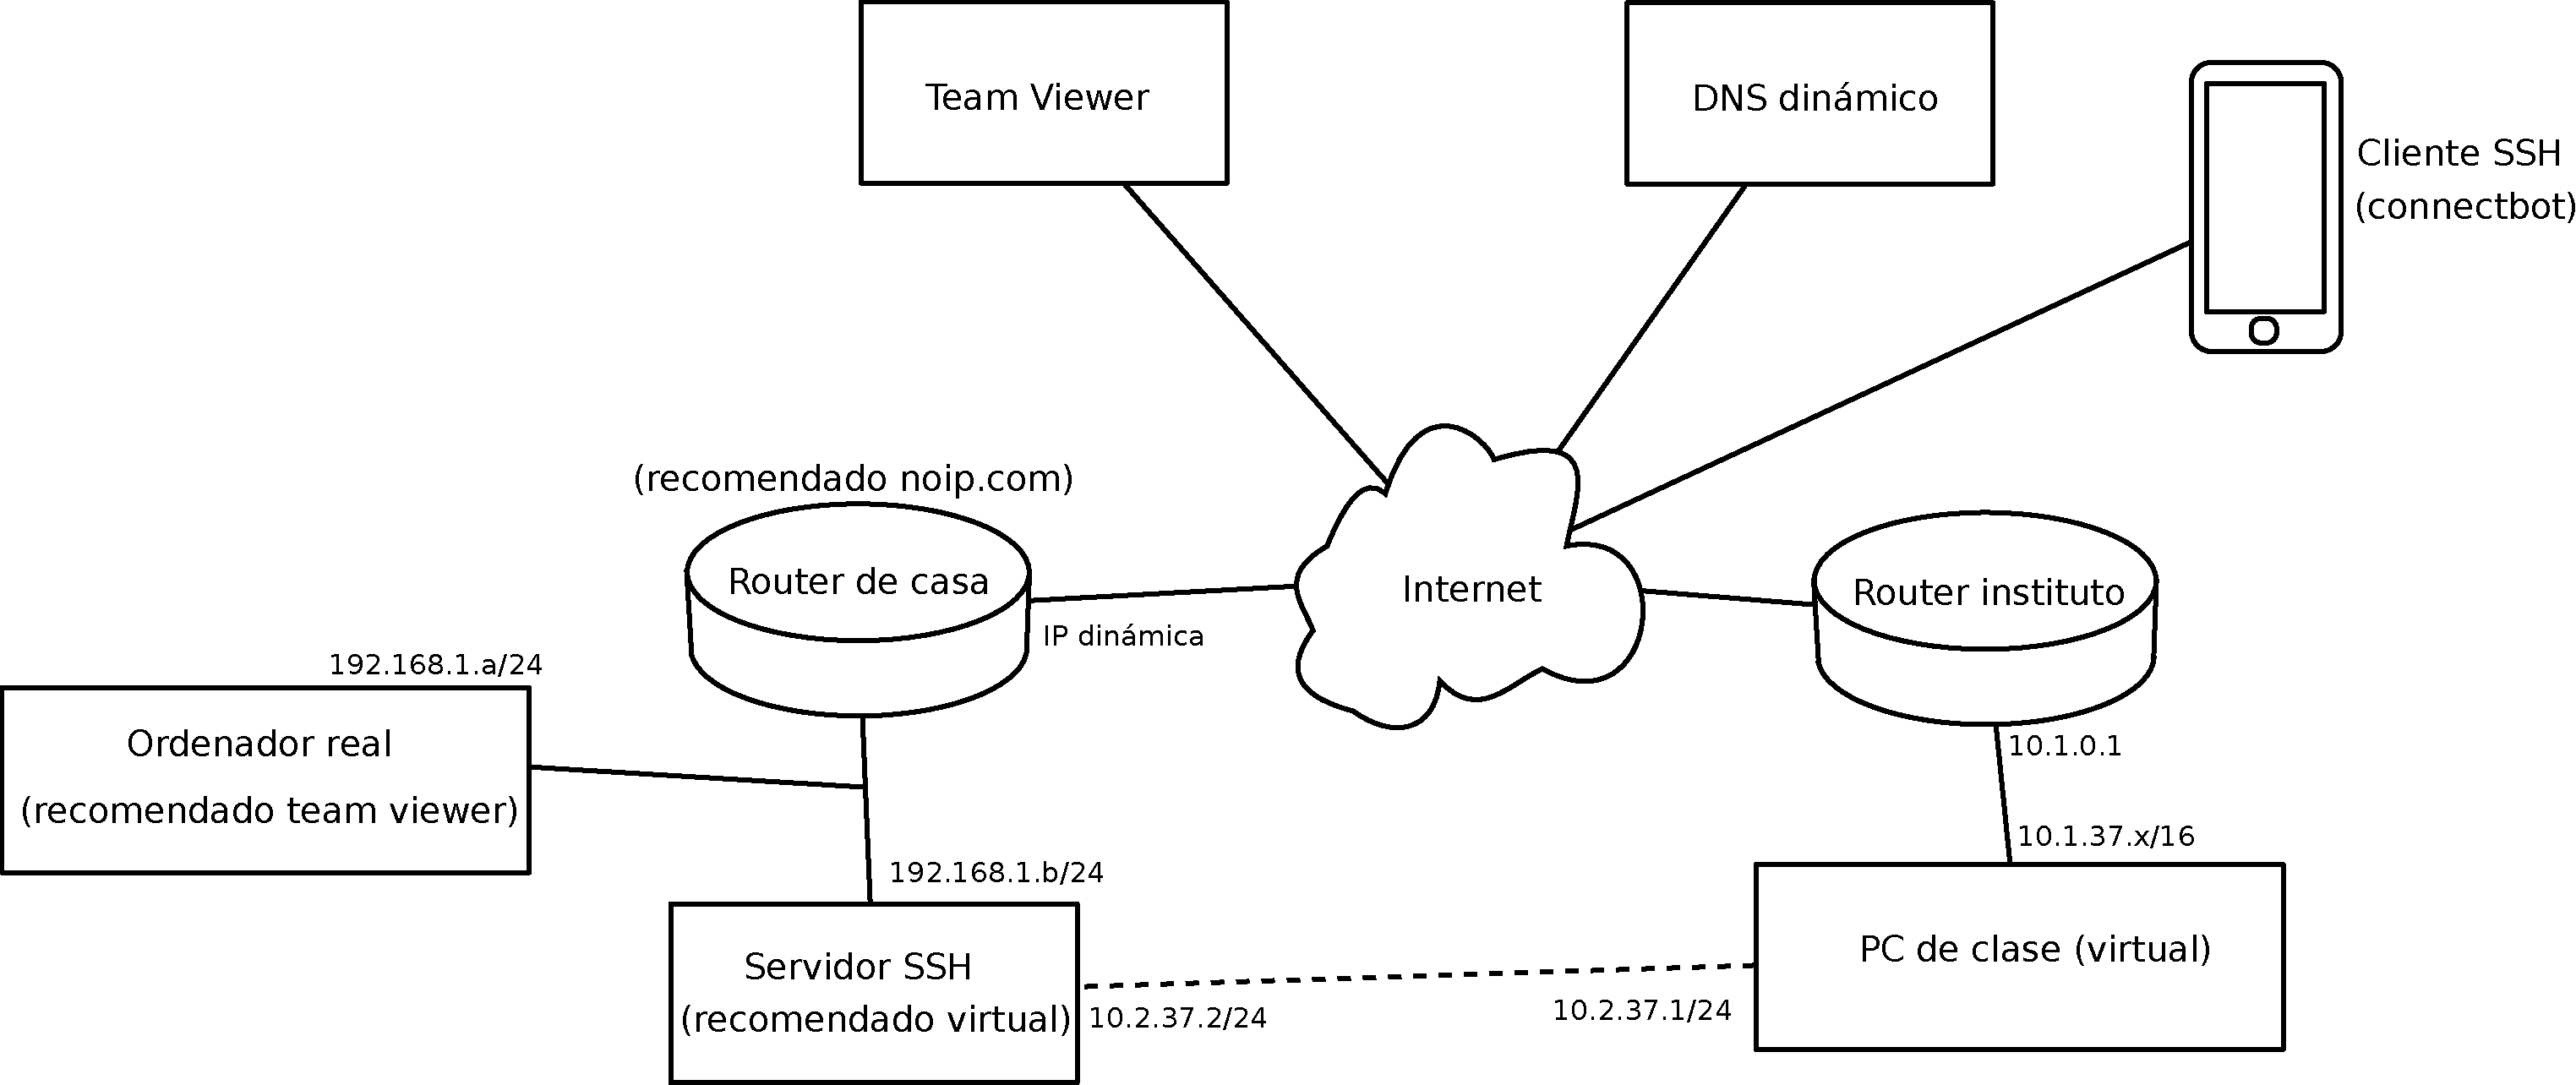
\includegraphics[width=.9\textwidth]{./media/practica-vpn-general.pdf}
  \end{center}
  \caption{Diagrama general de la práctica}\label{fig:diagrama-general}
\end{figure}


\begin{itemize}
\item Se creará una VPN entre un ordenador del aula y un ordenador en el domicilio del estudiante.
\item Se supone que el ordenador real del domicilio es Windows
\item Las máquinas virtuales serán Linux
\item El ordenador en el domicilio será una máquina virtual (para mayor seguridad)
\item La práctica se puede realizar fuera de clase, utilizando un móvil como punto de acceso desde un ordenador  
\end{itemize}

\section{(Opcional) Team Viewer en el ordenador real de casa}
Durante el desarrollo de la práctica, puede ser necesario reconfigurar los ordenadores de casa o el propio router. Para ello hay varias opciones
\begin{enumerate}
\item El alumno configura su casa y luego acude a clase a configurar el resto. Si tiene que hacer algún cambio en casa vuelve allí.
\item La práctica se hace por parejas. Un alumno está en su casa y otro en el instituto.
  
\item Se configura solo el \textit{Remote Desktop} al ordenador real, y se abre el puerto \texttt{3389} para poder acceder desde Internet.
\item \textbf{(Preferida)} Se instala Team Viewer en casa, que no necesita abrir ningún puerto, y se controla el PC real de casa en caso necesario. 
\end{enumerate}

\begin{figure}[h]
  \begin{center}
    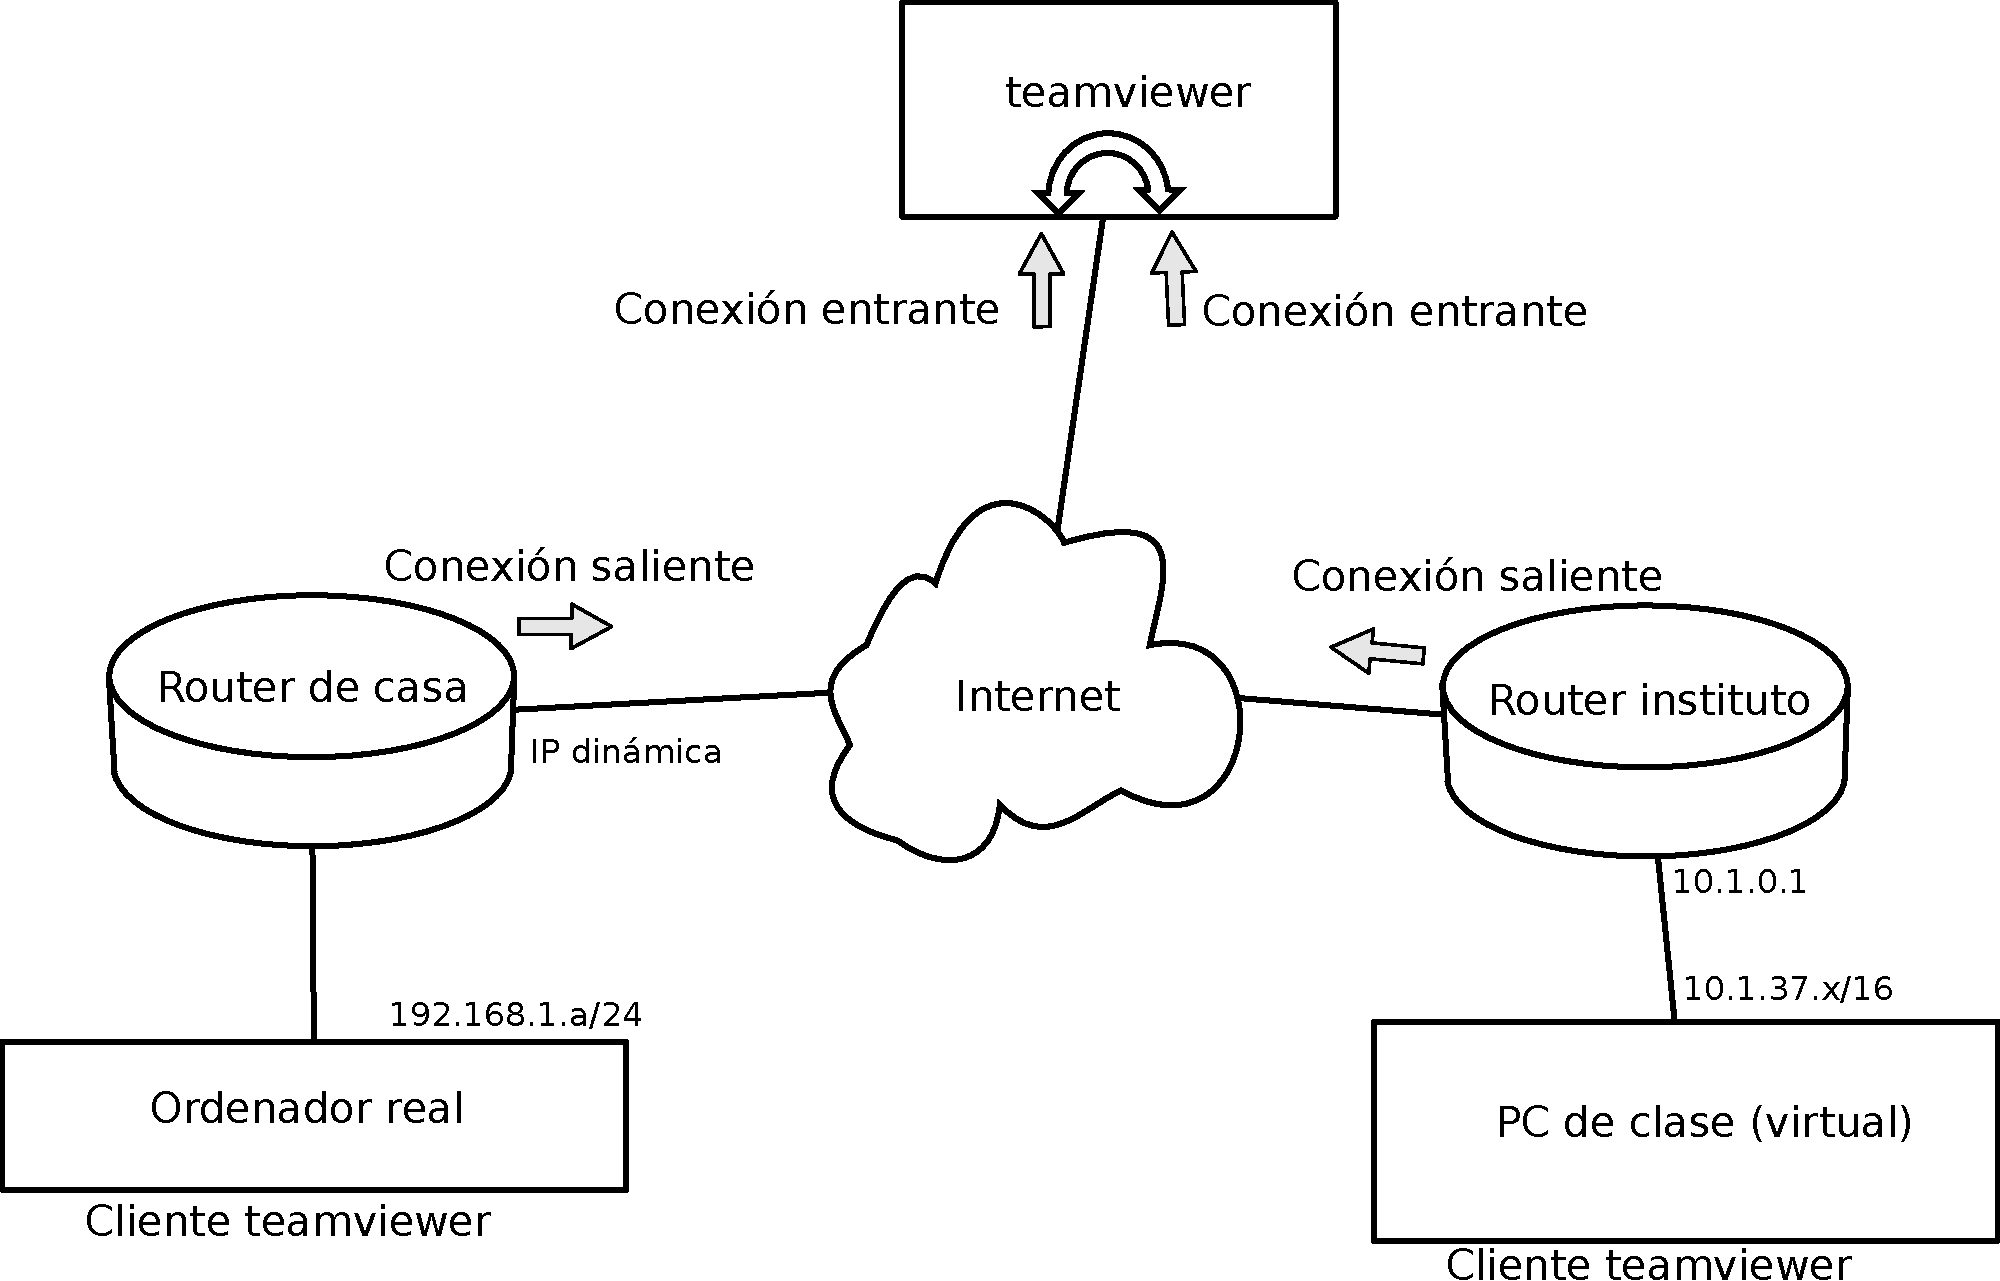
\includegraphics[width=.9\textwidth]{./media/practica-vpn-teamviewer.pdf}
  \end{center}
  \caption{Diagrama general de la práctica}\label{fig:diagrama-general}
\end{figure}

\begin{Aviso}
  \begin{itemize}
  \item Si se opta por utilizar \texttt{Remote Desktop}, se debe utilizar una contraseña suficientemente segura.
  \item Se recomienda que el puerto externo de \texttt{Remote Desktop} no sea \texttt{3389}, para evitar algunos ataques.
  \end{itemize}
\end{Aviso}

\section{IP externa del router de casa}
Hay varias opciones para conocer la IP externa del router de casa:
\begin{enumerate}
\item Desde un navegador de casa, visitar la página \url{http://www.cualesmiip.com/}. Dará la IP de ese momento, que puede cambiar en pocas horas.
\item \textbf{(Preferida)} Crear una cuenta de un \enlace{https://es.wikipedia.org/wiki/DNS\_din\%C3\%A1mico}{DNS dinámico}, como \url{http://www.noip.com}. Después, ejecutar un programa en la LAN que comunique automáticamente al DNS vuestra dirección IP
  \begin{itemize}
  \item Algunos routers traen ya este programa instalado (\enlace{https://www.redeszone.net/redes/host-en-no-ip-manual-para-crear-un-dynamic-dns-con-no-ip/}{enlace a ejemplo})
  \item También se puede instalar un \enlace{https://www.noip.com/download?page=win}{programa para actualizar la IP} en la máquina real Windows 
  \end{itemize}
\end{enumerate}

\begin{figure}[h]
  \begin{center}
    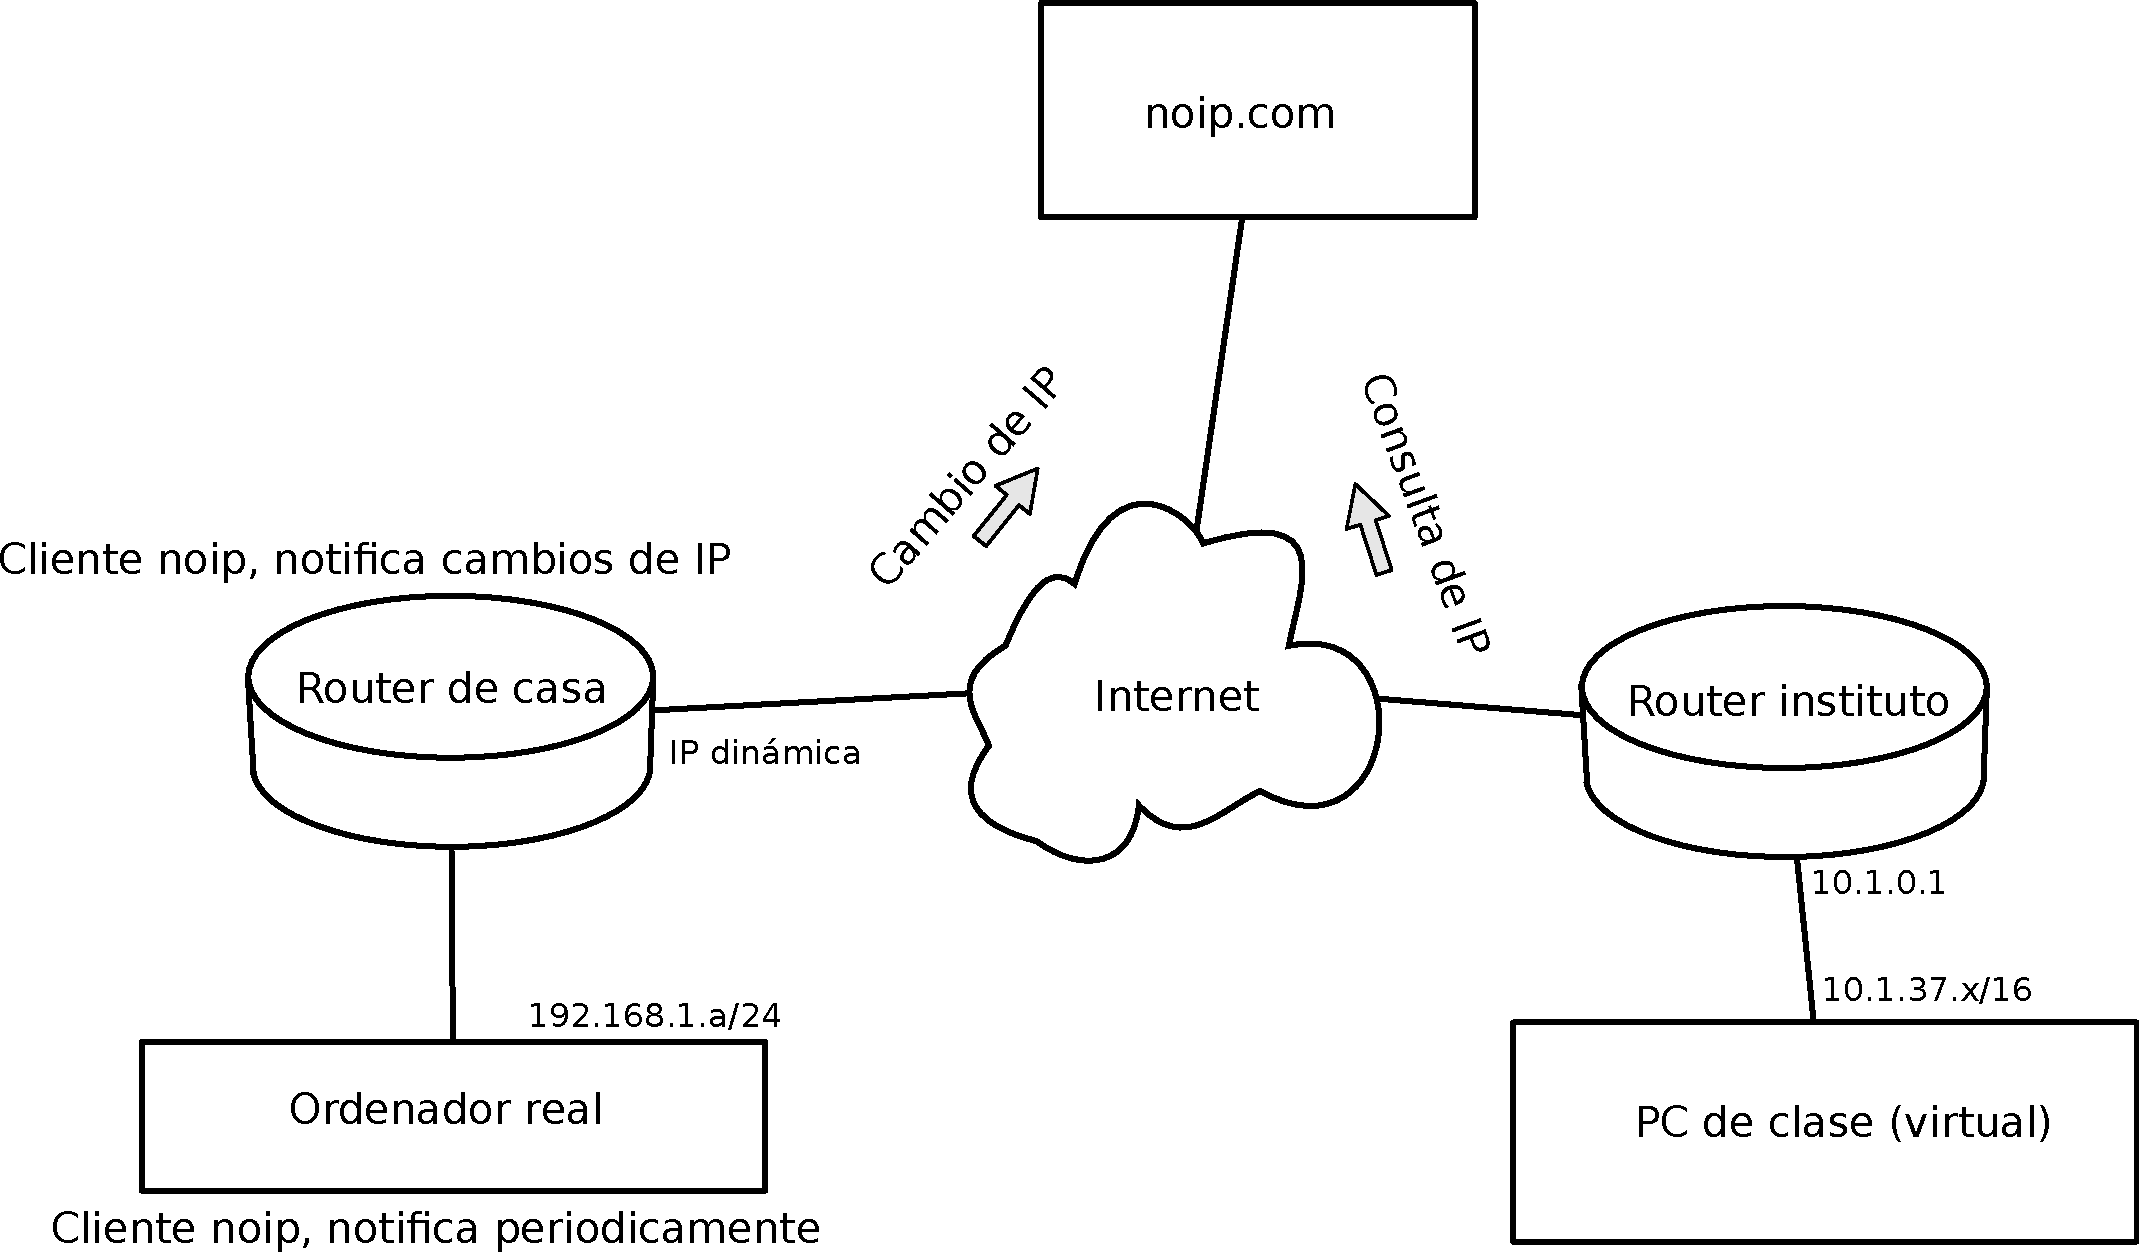
\includegraphics[width=.9\textwidth]{./media/practica-vpn-dyndns.pdf}
  \end{center}
  \caption{Funcionamiento DNS dinámico}\label{fig:dns-dinamico}
\end{figure}


\section{Servidor SSH}
\begin{itemize}
\item Se recomienda que sea una máquina virtual Linux
\item Debe configurarse con IP fija dentro de la LAN de casa
\item Se instalará openssh-server, con la configuración por defecto
\item En el router, debe abrirse un puerto para el servidor SSH
  \begin{itemize}
  \item Cada router de cada compañía telefónica es distinto
  \item Los clientes de telefónica utilizan el \enlace{https://comunidad.movistar.es/t5/Bienvenida-y-Noticias/C\%C3\%B3mo-abrir-los-puertos-de-tu-Router/td-p/1537794}{Portal Alejandra}.
  \end{itemize}
\item Para comprobar que se ha abierto correctamente, puede utilizarse una \enlace{https://play.google.com/store/apps/details?id=org.connectbot\&hl=en\_US}{aplicación de cliente SSH} desde el móvil, accediendo por 3G (sin wifi)
\end{itemize}

\begin{Aviso}
  \begin{itemize}
  \item Las contraseñas del servidor SSH deben ser \textbf{seguras}. Estará expuesto a Internet.
  \item Se recomienda que el puerto abierto para SSH no sea el \texttt{22}, para evitar algunos ataques.
  \item Se debe contar con el\textbf{permiso de los padres} para modificar el router de casa.
  \end{itemize}
\end{Aviso}


\section{VPN}
El servidor SSH se debe configurar con las siguientes opciones en su fichero \texttt{/etc/ssh/sshd\_config}:

\begin{listadoshell}{Opciones para el servidor SSH}{lst:sshdconfig}
  PermitRootLogin yes
  PermitTunnel yes
\end{listadoshell}

\begin{enumerate}
\item Se creará una conexión VPN entre el ordenador del aula y el servidor SSH
\item Se asignarán las siguientes direcciones IP en las interfaces TUN
  \begin{itemize}
  \item Aula: \texttt{10.2.37.1/24}
  \item Servidor SSH: \texttt{10.2.37.2/24}
  \end{itemize}
\end{enumerate}

Tras esto, debe haber comunicación directa (1 salto IP) entre el servidor SSH y el PC del centro.


\section{Acceso a la LAN desde el centro}
\begin{enumerate}
\item El ordenador de clase añadirá una ruta para acceder a la red \texttt{192.168.0.0/16} a través de \texttt{10.2.37.1}

  \begin{listadoshell}{Enrutamiento desde el aula a casa}{lst:enrutamiento}
    route add -net 192.168.0.0/16 gw 10.2.37.2
  \end{listadoshell}
  
\item El servidor SSH realizará NAT, de forma que el PC de clase sea enmascarado por el servidor SSH, y el resto de PCs de la LAN de casa puedan responderle
  
  \begin{listadoshell}{NAT para acceder a la LAN}{lst:nat}
    sudo iptables -t nat -A POSTROUTING -s 10.2.37.0/24 -o eth0 -j MASQUERADE
  \end{listadoshell}
  

\end{enumerate}

Como resultado, el ordenador de clase debe acceder a todos los ordenadores de la LAN de casa.

\begin{figure}[h]
  \begin{center}
    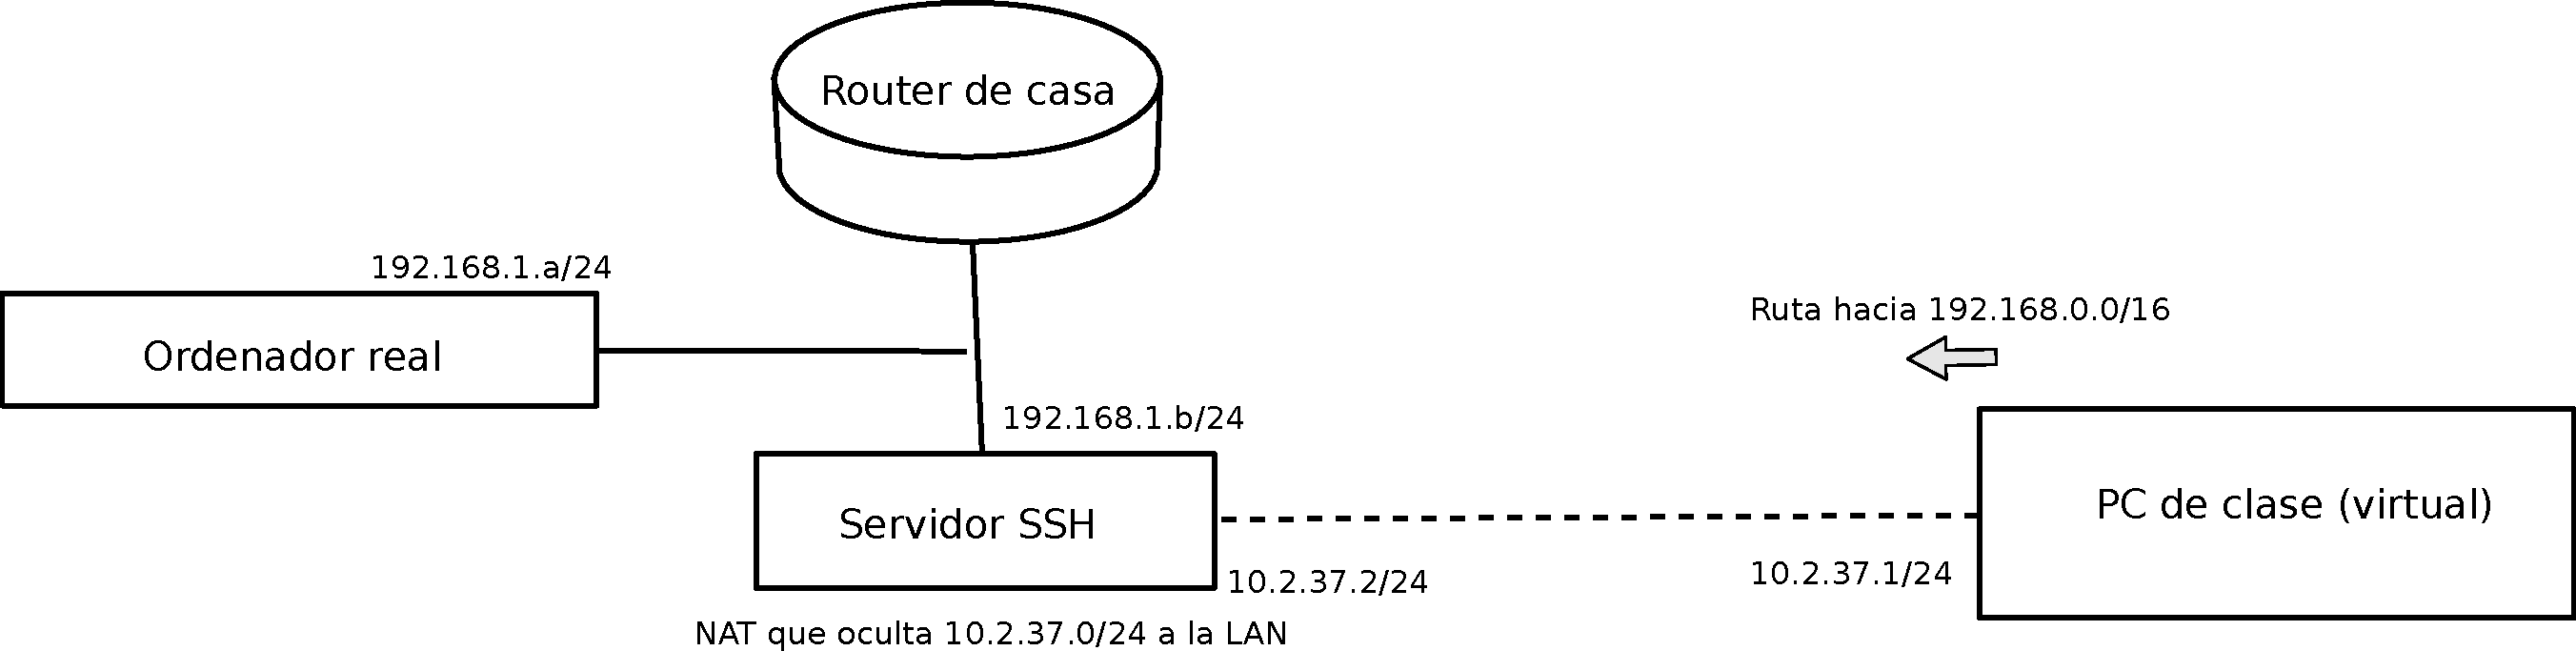
\includegraphics[width=.9\textwidth]{./media/practica-vpn-nat.pdf}
  \end{center}
  \caption{Enrutamiento y NAT para acceso a red de casa}\label{fig:enrutamiento-y-nat}
\end{figure}

\section{Normas de entrega}
\begin{itemize}
  
\item La entrega se realizará en el Áula Virtual
\item Se entregará un fichero PKT que pueda abrirse con la versión 7.1 de Packet Tracer.
\item Los equipos identificarán en su etiqueta su IP, y su pertenencia a algún departamento o función.
\end{itemize}

\section{Qué se valorará}
\begin{itemize}
\item Que se respeten los dominios de difusión (\textbf{3} puntos)
  \begin{itemize}
  \item Se entiende que dos equipos \textit{no comparten dominio de difusión} si un broadcast de Ethernet (por ejemplo, ARP) no consigue viajar entre ellos en ninguno de los sentidos.
  \end{itemize}
\item Que se incluyan etiquetas identificativas en cada equipo (\textbf{1.5} puntos)  
\item Que los departamentos puedan comunicarse a través de la capa 3 (\textbf{2} puntos)
\item Que se rellene correctamente la tabla de documentación de la red (\textbf{2} puntos)
\item \textbf{No se valorará} el ejercicio si las direcciones IP no son de la subred \texttt{10.N.0.0/16}.
\end{itemize}



\end{document}
